\chapter{Gobbled Lstlistings examples:}\label{results}

\section{Gobbled lstlistings}

\begin{enumerate}
    \item \lstinline[language=bash]{mkdir ~/my-project}

    \item copy whl file in \lstinline{my-project/dist}

    \item Python 3.9 local pyenv

    \begin{lstlisting}[language=bash, title={small Execute in: bash}]
    # @ ~/my-project

    pyenv local 3.9.6
    python -m venv venv
    . venv/scripts/activate    
    \end{lstlisting}

    \item install and set up \lstinline{FLASK_APP}

    \begin{lstlisting}[language=bash, title={small Execute in: bash}]
    # @ ~/my-project (venv)

    pip install package-name-1.0.1-py3-none-any.whl
    export FLASK_APP=package-name
    flask run
    \end{lstlisting}

\end{enumerate}

\section{Design}

We used Paletton. \href{https://paletton.com/#uid=53n0u0kmgAe6fUpfzJrtUwl-jnK}{chosen color scheme}。\footnote{\label{paletton}Paletton color scheme: \href {https://paletton.com/\#uid=53n0u0kmgAe6fUpfzJrtUwl-jnK}{\path{https://paletton.com/#uid=53n0u0kmgAe6fUpfzJrtUwl-jnK}}}

See in fig. \ref{fig:color-palette}.

\begin{figure}[bh]
\centering
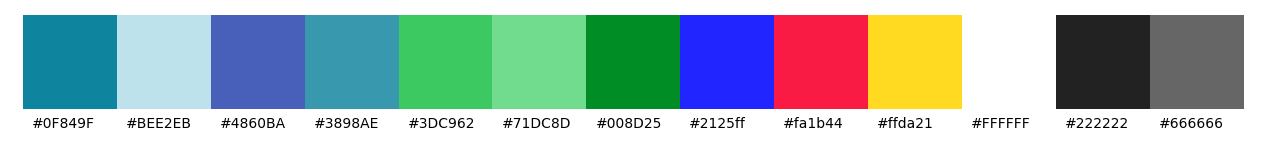
\includegraphics[width=0.6\linewidth]{figures/color-palette.png}
\caption{Color palette}
\label{fig:color-palette}
\end{figure}


%%%%%%%%%%%%%%%%%%%%%%%%%
%%%%%%%%%%%%%%%%%%%%%%%%%
%%%%%%%%%%%%%%%%%%%%%%%%%
